\documentclass[11pt]{article}
\usepackage[margin=1in]{geometry}
\usepackage{amsmath,amssymb,amsthm}
\usepackage{graphicx,float}
\usepackage{lmodern}
\usepackage[T1]{fontenc}
\usepackage{xcolor,framed,booktabs,listings,microtype,array}
\usepackage[colorlinks=true,linkcolor=blue!60!black,urlcolor=blue!60!black]{hyperref}

\definecolor{shadecolor}{RGB}{240,244,250}
\definecolor{codebg}{RGB}{248,248,248}
\lstset{language=Python,basicstyle=\ttfamily\footnotesize,backgroundcolor=\color{codebg},
  keywordstyle=\color{blue!70!black},commentstyle=\color{green!45!black},stringstyle=\color{orange!80!black},
  frame=single,rulecolor=\color{gray!40},breaklines=true,showstringspaces=false,columns=fullflexible}

\newcommand{\R}{\mathbb{R}}
\newcommand{\T}{^{\mathsf T}}
\newcommand{\ones}{\mathbf{1}}
\newcommand{\answer}[1]{\begin{shaded}\noindent\textbf{Answer.} #1\end{shaded}}
\newtheorem*{lemma*}{Lemma}
\newtheorem*{claim*}{Claim}

\title{Optimization --- Homework 3 \\ \large Solutions}
\author{Mitchel Carson}
\date{\today}

\begin{document}
\maketitle

\noindent\textit{Conventions.} Vectors are columns; inequalities between vectors are componentwise; $A_j$ is the $j$-th column of $A$ and $a_i\T$ its $i$-th row. For a minimisation LP I use the standard primal--dual dictionary
\begin{center}\renewcommand{\arraystretch}{1.15}
\begin{tabular}{@{}ll@{\qquad\qquad}ll@{}}\toprule
\multicolumn{2}{c}{\textbf{Primal} (min $c\T x$)} & \multicolumn{2}{c}{\textbf{Dual} (max $p\T b$)}\\ \midrule
constraint $a_i\T x\ge b_i$ & & $p_i\ge0$ &\\
constraint $a_i\T x\le b_i$ & & $p_i\le0$ &\\
constraint $a_i\T x= b_i$ & & $p_i$ free &\\[2pt]
variable $x_j\ge0$ & & $p\T A_j\le c_j$ &\\
variable $x_j\le0$ & & $p\T A_j\ge c_j$ &\\
variable $x_j$ free & & $p\T A_j= c_j$ &\\ \bottomrule
\end{tabular}\end{center}
and the three facts \emph{weak duality} ($p\T b\le c\T x$ for any feasible pair), \emph{strong duality} (if either problem has an optimal solution so does the other, with equal values), and \emph{complementary slackness} (a feasible pair is optimal iff $p_i(a_i\T x-b_i)=0$ for all $i$ and $(c_j-p\T A_j)x_j=0$ for all $j$).

%======================================================================
\section*{Problem 1. Computing a dual}

The LP is
\[
\begin{array}{rrcrcrcrcl}
\min & x_1 &-& x_2\\
\text{s.t.} & 2x_1&+&3x_2&-&x_3&+&x_4&\le&0\\
& 3x_1&+&x_2&+&4x_3&-&2x_4&\ge&3\\
& -x_1&-&x_2&+&2x_3&+&x_4&=&6\\
& \multicolumn{9}{l}{x_1\le0,\qquad x_2,x_3\ge0,\qquad x_4\ \text{free}.}
\end{array}
\]
In matrix form: $c=(1,-1,0,0)\T$, $b=(0,3,6)\T$,
$A=\begin{pmatrix}2&3&-1&1\\3&1&4&-2\\-1&-1&2&1\end{pmatrix}$.
Note that $x_4$ carries no sign restriction, so it is a free variable.

\paragraph{Derivation via the Lagrangian.} Attach a multiplier $p_i$ to each of the three general constraints and keep the sign constraints on $x$ explicit. Define
\[
g(p)=\min_{x_1\le0,\;x_2,x_3\ge0,\;x_4\in\R}\Big[c\T x+p\T(b-Ax)\Big]
=p\T b+\min_{x_1\le0,\;x_2,x_3\ge0,\;x_4\in\R}\sum_{j=1}^4\big(c_j-p\T A_j\big)x_j .
\]
\emph{Signs of $p$.} We want $g(p)$ to be a lower bound on the primal optimum, i.e.\ $p\T(b-Ax)\le0$ for every primal-feasible $x$. Row~1 has $b_1-a_1\T x\ge0$, so we need $p_1\le0$; row~2 has $b_2-a_2\T x\le0$, so $p_2\ge0$; row~3 has $b_3-a_3\T x=0$, so $p_3$ is free.

\emph{Constraints on $p$.} The inner minimum is $-\infty$ unless each term is bounded below over the allowed sign of $x_j$:
$x_1\le0$ requires $c_1-p\T A_1\le0$; \ $x_2,x_3\ge0$ require $c_j-p\T A_j\ge0$; \ $x_4$ free requires $c_4-p\T A_4=0$. When these hold the minimum is $0$ and $g(p)=p\T b=0p_1+3p_2+6p_3$. Maximising the lower bound gives the dual, in agreement with the dictionary above.

\answer{
\[
\begin{array}{rrcrcrcl}
\max & \multicolumn{5}{l}{3p_2+6p_3}\\
\text{s.t.} & 2p_1&+&3p_2&-&p_3&\ge&\phantom{-}1\qquad(x_1\le0)\\
& 3p_1&+&p_2&-&p_3&\le&-1\qquad(x_2\ge0)\\
& -p_1&+&4p_2&+&2p_3&\le&\phantom{-}0\qquad(x_3\ge0)\\
& p_1&-&2p_2&+&p_3&=&\phantom{-}0\qquad(x_4\text{ free})\\
& \multicolumn{7}{l}{p_1\le0,\qquad p_2\ge0,\qquad p_3\ \text{free}.}
\end{array}
\]
(Equivalently, substituting $q_1=-p_1\ge0$ gives a version with all sign-constrained multipliers nonnegative.)}

\paragraph{Going further: what are the optimal values?} The problem only asks for the dual, but it is instructive to solve the pair.

\emph{The dual is infeasible.} The equality gives $p_3=2p_2-p_1$. Substituting into the third constraint: $-p_1+4p_2+2(2p_2-p_1)=-3p_1+8p_2\le0$. But $p_1\le0$ and $p_2\ge0$ make both $-3p_1$ and $8p_2$ nonnegative, so $p_1=p_2=0$ and hence $p_3=0$. Then the first constraint reads $0\ge1$, which is false.

\emph{The primal is feasible and unbounded.} The point $x^0=(0,0,2,2)$ is feasible: the rows evaluate to $0\le0$, $4\ge3$, $6=6$. The direction $d=(-1,0,1,-3)$ satisfies $Ad=(-6,\,7,\,0)$, $d_1\le0$, $d_2,d_3\ge0$, so $x^0+\theta d$ is feasible for every $\theta\ge0$, while the cost is $c\T(x^0+\theta d)=-\theta\to-\infty$ (Figure~\ref{fig:ray}).

This is exactly what duality predicts: by weak duality any dual-feasible $p$ would give a finite lower bound on the primal, so an unbounded primal \emph{forces} an infeasible dual. Both facts are confirmed numerically in Appendix~\ref{app:code}.

\begin{figure}[H]\centering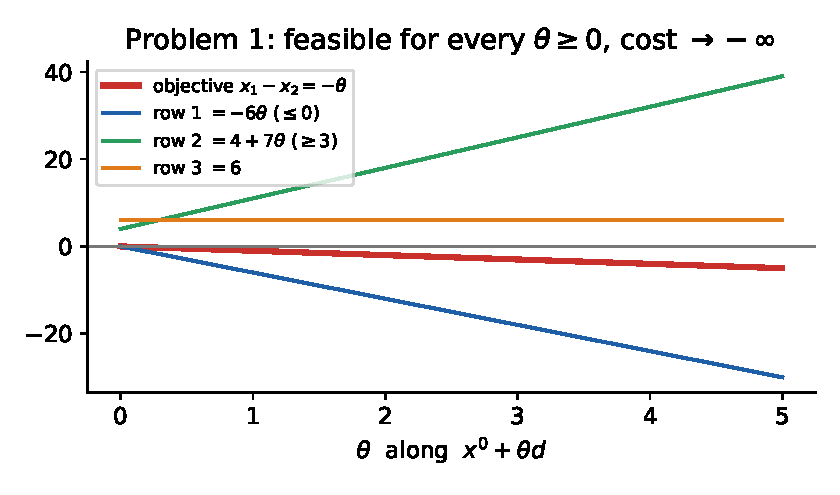
\includegraphics[width=.6\textwidth]{figures/p1_ray.pdf}
\caption{Along $x^0+\theta d$ all three constraints remain satisfied while the objective decreases without bound.}\label{fig:ray}\end{figure}

%======================================================================
\section*{Problem 2. A theorem of the alternative}

For a matrix $A\in\R^{m\times n}$ we show the equivalence of
\begin{enumerate}
\item[(i)] $Ax\ge0$ and $x\ge0$ imply $x_1=0$;
\item[(ii)] there exists $p\ge0$ with $p\T A\le0$ and $p\T A_1<0$.
\end{enumerate}

\begin{proof}[Proof of (ii) $\Rightarrow$ (i)]
Let $p$ be as in (ii) and let $x$ satisfy $Ax\ge0$, $x\ge0$. Since $p\ge0$ and $Ax\ge0$, we have $p\T Ax\ge0$. On the other hand
\[
p\T A x=\sum_{j=1}^n (p\T A_j)\,x_j ,
\]
and every term is $\le0$ because $p\T A_j\le0$ and $x_j\ge0$. A sum of nonpositive terms that is $\ge0$ must have every term equal to zero; in particular $(p\T A_1)x_1=0$. Since $p\T A_1<0$ strictly, $x_1=0$.
\end{proof}

\begin{proof}[Proof of (i) $\Rightarrow$ (ii)]
Consider the linear program
\[
\text{(P)}\qquad \min\ -x_1\quad\text{s.t.}\quad Ax\ge0,\quad x\ge0 .
\]
It is feasible ($x=0$). Statement (i) says every feasible $x$ has objective value $-x_1=0$, so (P) has an optimal solution, with optimal value $0$. Using the dictionary (constraints ``$\ge$'' give $p\ge0$; variables $x\ge0$ give $p\T A_j\le c_j$; here $c=-e_1$ and the right-hand side is $b=0$), the dual is
\[
\text{(D)}\qquad \max\ p\T 0=0\quad\text{s.t.}\quad p\ge0,\quad p\T A_1\le-1,\quad p\T A_j\le0\ \ (j=2,\dots,n).
\]
By strong duality, since (P) has an optimal solution, so does (D); in particular (D) is \emph{feasible}. Any feasible $p$ satisfies $p\ge0$, $p\T A\le0$ and $p\T A_1\le-1<0$, which is (ii).
\end{proof}

\answer{(i) $\Leftrightarrow$ (ii). The easy direction is a one-line ``multiply and add'' argument; the hard direction is strong LP duality applied to $\min\{-x_1:Ax\ge0,\,x\ge0\}$, whose dual is a pure feasibility problem.

\emph{Remark on the strict inequality.} The dual produces $p\T A_1\le-1$, which looks stronger than $p\T A_1<0$, but the two are equivalent: the conditions $p\ge0$, $p\T A\le0$ are homogeneous, so any $p$ with $p\T A_1<0$ can be rescaled to $p/|p\T A_1|$, which has $p\T A_1=-1$. This rescaling trick is the standard way to convert a strict inequality (which LPs cannot express) into a non-strict one.

\emph{Remark on the structure.} If (i) fails there is a feasible $x$ with $x_1>0$; then $\theta x$ is feasible for all $\theta\ge0$, (P) is unbounded, and weak duality forces (D) to be infeasible, so (ii) fails. Thus exactly one of ``there is $x\ge0$ with $Ax\ge0$, $x_1>0$'' and ``(ii)'' holds, which is the usual form of a theorem of the alternative.}

\begin{figure}[H]\centering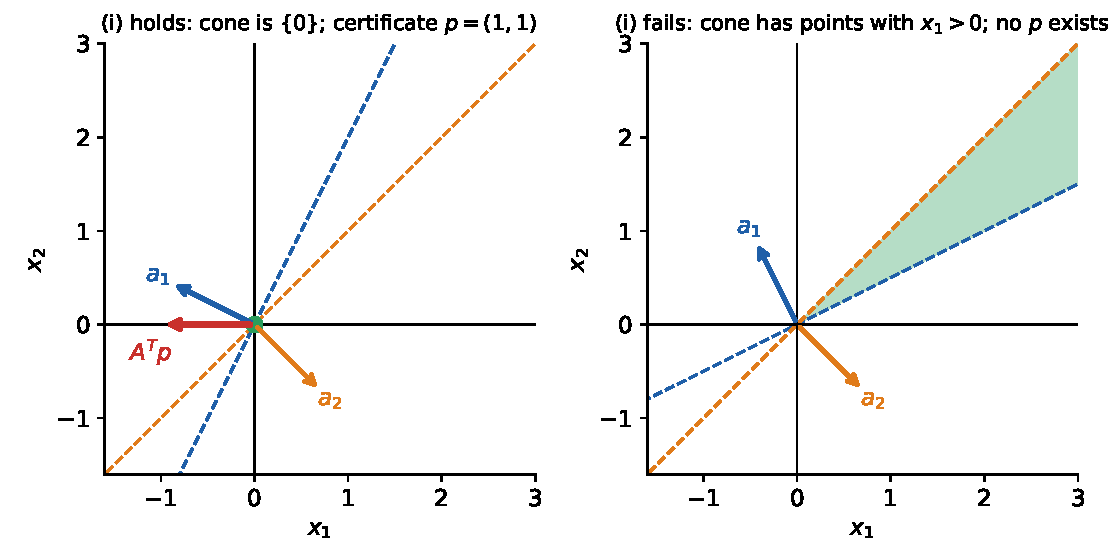
\includegraphics[width=.85\textwidth]{figures/p2_alternatives.pdf}
\caption{Green: the cone $\{x\ge0,\ Ax\ge0\}$; dashed lines: $a_i\T x=0$. Left, $A=\big(\begin{smallmatrix}-2&1\\1&-1\end{smallmatrix}\big)$: the cone is $\{0\}$ and $p=(1,1)$ gives $A\T p=(-1,0)$, nonpositive with a strictly negative first entry. Right, $A=\big(\begin{smallmatrix}-1&2\\1&-1\end{smallmatrix}\big)$: the cone contains points with $x_1>0$, e.g.\ $x=(1.5,1)$, so no certificate $p$ can exist.}\end{figure}

\noindent\emph{Numerical check.} For 2000 random integer matrices I tested (i) and (ii) independently by LP; they agreed in every case (1140 both true, 860 both false, 0 disagreements; Appendix~\ref{app:code}).

%======================================================================
\section*{Problem 3. An infeasible system has a small infeasible subsystem}

Let $A\in\R^{m\times n}$ with $m=500$, $n=100$, and suppose $\{x:Ax\le b\}=\emptyset$. We show that some subset of at most $n+1=101$ of the inequalities $a_i\T x\le b_i$ is already infeasible.

\subsection*{Proof via duality and complementary slackness (the hinted route)}

\paragraph{Step 1: an LP that measures infeasibility.} Introduce one extra variable $t$ and consider
\[
\text{(P)}\qquad \min_{x\in\R^n,\;t\in\R}\ t\qquad\text{s.t.}\qquad a_i\T x-t\le b_i,\quad i=1,\dots,m .
\]
For fixed $x$ the best $t$ is $\max_i(a_i\T x-b_i)$, the worst constraint violation at $x$. (P) is feasible (take any $x$ and $t$ large). Because $Ax\le b$ has no solution, every feasible $(x,t)$ has $t\ge\max_i(a_i\T x-b_i)>0$; so (P) is bounded below by $0$. A feasible LP with bounded objective has an optimal solution $(x^\star,t^\star)$, and since $x^\star$ violates some inequality, $t^\star>0$.

\paragraph{Step 2: the dual.} Write the constraints as $-a_i\T x+t\ge-b_i$ with multipliers $p_i\ge0$. Both $x$ and $t$ are free, so the dual constraints are equalities:
\[
\text{(D)}\qquad \max\ -b\T p\qquad\text{s.t.}\qquad A\T p=0,\quad \ones\T p=1,\quad p\ge0 .
\]
By strong duality (D) has an optimal solution and its optimal value is $t^\star>0$.

\paragraph{Step 3: a sparse optimal dual solution.} (D) is an LP in \emph{standard form}: nonnegative variables $p\in\R^{m}$ and $n+1=101$ equality constraints. Its feasible set contains no line (it lies in $p\ge0$), so it has extreme points, and an LP with an optimal solution over such a polyhedron has an optimal solution $p^\star$ that is an extreme point, i.e.\ a basic feasible solution. In a basic feasible solution of a standard-form LP the columns of the equality matrix corresponding to positive variables are linearly independent; these columns live in $\R^{n+1}$, so
\[
S=\{i:p_i^\star>0\}\qquad\text{satisfies}\qquad |S|\le n+1=101 .
\]

\paragraph{Step 4: the subsystem indexed by $S$ is infeasible.} Consider the LP $(\mathrm P_S)$ obtained from (P) by keeping only the constraints $i\in S$, and its dual $(\mathrm D_S)$, which is (D) with variables $(p_i)_{i\in S}$ only.
\begin{itemize}
\item $(x^\star,t^\star)$ is feasible for $(\mathrm P_S)$, since it satisfies \emph{all} $m$ constraints.
\item $p^\star_S=(p_i^\star)_{i\in S}$ is feasible for $(\mathrm D_S)$: deleting zero entries does not change $\sum_ip_i^\star a_i=0$ or $\sum_ip_i^\star=1$.
\item Complementary slackness holds for this pair. For the original optimal pair it gives $p_i^\star\,(b_i-a_i\T x^\star+t^\star)=0$ for all $i$, so every constraint $i\in S$ is tight at $(x^\star,t^\star)$; the conditions attached to the free variables are the dual equalities, which hold.
\end{itemize}
A primal-feasible and dual-feasible pair satisfying complementary slackness is optimal. Hence the optimal value of $(\mathrm P_S)$ is $t^\star>0$: even the best $x$ violates some inequality in $S$ by $t^\star$. Therefore $\{x:a_i\T x\le b_i,\ i\in S\}=\emptyset$, with $|S|\le101$.

\emph{Shortcut.} Weak duality alone finishes Step~4: $p^\star_S$ is feasible for $(\mathrm D_S)$ with value $-b_S\T p_S^\star=t^\star$, so every feasible point of $(\mathrm P_S)$ has $t\ge t^\star>0$. Complementary slackness adds the sharper information that the value is \emph{exactly} $t^\star$ and that the constraints in $S$ are all tight at $x^\star$.

\answer{There is always an infeasible subsystem of at most $n+1=101$ inequalities: the support of a basic optimal solution of the dual of the ``minimise the worst violation'' LP. Complementary slackness tells us precisely which inequalities matter: the ones that are tight at the point of least violation \emph{and} carry positive dual weight. The other $\ge399$ inequalities are irrelevant to the infeasibility. Nothing is special about $500$ and $100$: for $m$ inequalities in $n$ variables the bound is $\min\{m,\,n+1\}$.}

\subsection*{A second proof via Farkas' lemma (no optimisation needed)}
\begin{lemma*}[Farkas, inequality form]
$\{x:Ax\le b\}=\emptyset$ if and only if there is $p\ge0$ with $A\T p=0$ and $b\T p<0$.
\end{lemma*}
\noindent(The ``if'' direction is immediate: a solution $x$ would give $0=p\T Ax\le p\T b<0$.) Given infeasibility, rescale the certificate so that $b\T p=-1$. Then the polyhedron
\[
Q=\{p\in\R^m:\ A\T p=0,\ b\T p=-1,\ p\ge0\}
\]
is nonempty, in standard form, with $n+1$ equality constraints. A nonempty standard-form polyhedron has a basic feasible solution $\bar p$, with at most $n+1$ positive entries. Let $S$ be its support. Then $\sum_{i\in S}\bar p_ia_i=0$ and $\sum_{i\in S}\bar p_ib_i=-1<0$, so $\bar p_S$ is a Farkas certificate for the subsystem $S$, which is therefore infeasible by the easy direction of the lemma.

\emph{Why a BFS exists, constructively.} If the columns $\binom{a_i}{b_i}$, $i\in\operatorname{supp}(p)$, are linearly dependent, pick $z\ne0$ supported there with $\sum_iz_i\binom{a_i}{b_i}=0$ and (flipping sign if needed) some $z_i>0$. Moving to $p-\theta z$ keeps both equalities, and at $\theta=\min\{p_i/z_i:z_i>0\}$ it keeps $p\ge0$ while zeroing at least one more entry. Repeat until the columns are independent, which forces at most $n+1$ of them. This is the same argument that proves Carath\'eodory's theorem, and I ran it numerically below.

\subsection*{The bound $n+1$ is tight, and the geometric meaning}
In $\R^n$ take the $n+1$ inequalities $x_j\ge1$ ($j=1,\dots,n$) and $\sum_jx_j\le n-1$. Together they are infeasible ($\sum_j x_j\ge n$), but dropping $x_k\ge1$ leaves the feasible point $x=\ones-e_k$, and dropping the sum constraint leaves $x=\ones$. So no subset of size $n$ is infeasible, and $101$ cannot be replaced by $100$. Figure~\ref{fig:helly} shows $n=2$.

The contrapositive is \textbf{Helly's theorem for half-spaces}: \emph{if every $n+1$ of a finite family of half-spaces in $\R^n$ have a common point, then all of them do.} Applications: an infeasible scheduling/resource model with thousands of constraints always has a ``small'' explanation of at most $n+1$ conflicting requirements (an \emph{irreducible infeasible subsystem}, which solvers report for debugging); a linear classifier in $\R^n$ fails to separate a data set only if some $n+2$ points are already inseparable; minimax/Chebyshev fitting problems are determined by at most $n+1$ active data points.

\begin{figure}[H]\centering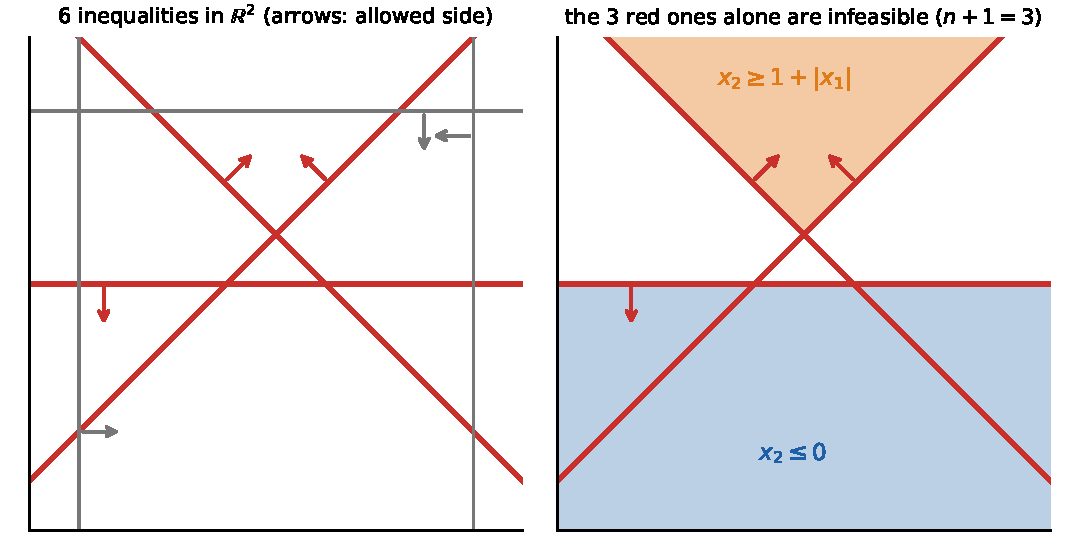
\includegraphics[width=.8\textwidth]{figures/p3_helly2d.pdf}
\caption{$n=2$. Left: six inequalities with no common point. Right: three of them, $x_2\le0$, $x_2\ge x_1+1$, $x_2\ge-x_1+1$, are already infeasible (the blue and orange regions are disjoint), with certificate $p=(1,\tfrac12,\tfrac12)$: $\sum p_ia_i=0$, $\sum p_ib_i=-1$. Any two of the three are feasible, so three is tight.}\label{fig:helly}\end{figure}

\subsection*{Numerical experiment}
I generated a random system with $m=500$, $n=100$ (Gaussian $A$ and $b$), which is infeasible with least worst-violation $t^\star=1.1517$. Solving (D) with a simplex method returns a vertex with exactly $101$ nonzero multipliers (Figure~\ref{fig:support}, left); the $101$-row subsystem was confirmed infeasible by an independent LP, and removing \emph{any} one of those 101 rows made it feasible, so this subset is minimal. Separately, starting from a dense Farkas certificate with 180 nonzeros, the reduction procedure above reached support 101 in 79 steps while preserving $A\T p=0$ and $b\T p=-1$ to within $2\times10^{-11}$ (Figure~\ref{fig:support}, right).

\begin{figure}[H]\centering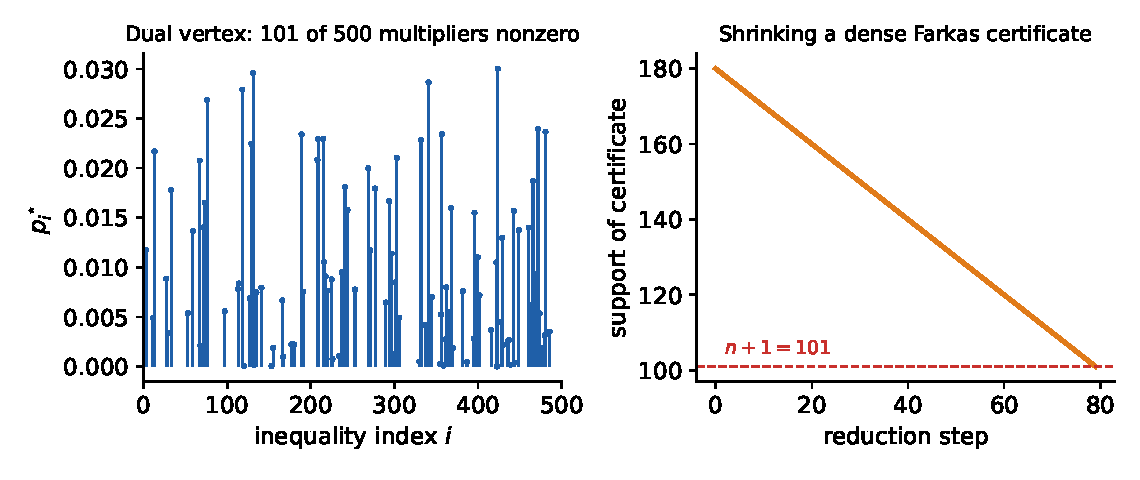
\includegraphics[width=.92\textwidth]{figures/p3_support.pdf}
\caption{Left: the optimal dual vertex $p^\star$; its support identifies the infeasible subsystem. Right: support size during the constructive reduction of a dense certificate.}\label{fig:support}\end{figure}

\noindent\emph{A caution from the experiment.} My first feasibility test passed a zero objective to the solver and checked for the ``infeasible'' status flag; on the full $500\times100$ system the solver instead returned ``status unknown'', which my code misread as feasible. I replaced it with the phase-1 LP (P) itself, declaring infeasibility iff $t^\star>0$; this LP is always feasible and (with a lower bound on $t$) bounded, so its answer is unambiguous. All results reported here use that test.

%======================================================================
\appendix
\section{Code and numerical checks}\label{app:code}
Figures were produced with \texttt{matplotlib} (\texttt{make\_figures.py}); LPs were solved with SciPy's HiGHS interface.

\lstinputlisting{verify.py}

\noindent Output:
\lstinputlisting[language={}]{verify_output.txt}

\end{document}
